\chapter{Betimsel İstatistiğin Gözden Geçirilmesi: Merkez, Yayılım, Dağılım ve Grafikler}
\label{ch:descriptive}

\begin{prismbox}[PrismLight]{Öğrenme çıktıları}
Bu bölümde frekans dağılımları, temel grafikler, merkezi eğilim ve yayılım
ölçüleri birlikte ele alınır. Amaç yalnız sayı hesaplamak değil, dağılımın
merkezini, değişkenliğini, biçimini ve olağandışı gözlemlerini açıklamaktır.
\end{prismbox}

\begin{prerequisitebox}
Veri türleri ve ölçme düzeyleri ayırt edilebilmelidir. Toplama, bölme,
karekök ve yüzde hesapları bu bölümde kullanılan temel matematiksel
işlemlerdir.
\end{prerequisitebox}

Değişken türleri ve ölçme düzeyleri Bölüm~\ref{sec:population-data-types}'te
tanımlanmıştır; bu bölümde grafik ve özet seçimi bu sınıflandırmaya dayanır.

\section{Önce veri yapısını tanımak}
\label{sec:descriptive-graphs}

Kategorik değişkenler frekans ve yüzdelerle; nicel değişkenler ise sıralı veri,
grafikler ve sayısal özetlerle incelenir. Bir grafik seçilirken değişkenin
ölçme düzeyi belirleyicidir. Keşfedici veri analizinin grafik ve sağlam
özetlere verdiği önem için bkz. \citet{tukey1977}.
Türkçe bir uygulamalı başvuru için ayrıca \citet{koklu2006} incelenebilir.

\begin{table}[H]
\centering
\caption{Değişken türüne göre grafik seçimi.}
\label{tab:graph-choice}
\begin{tabular}{p{0.27\textwidth}p{0.57\textwidth}}
\toprule
Veri yapısı & Önerilen grafik \\
\midrule
Tek kategorik değişken & Çubuk grafiği, Pareto grafiği \\
Tek nicel değişken & Histogram, nokta grafiği, kutu grafiği \\
İki nicel değişken & Saçılım grafiği \\
Nicel sonuç ve kategorik grup & Yan yana kutu grafikleri \\
İki kategorik değişken & Çapraz tablo, yığılmış çubuk veya mozaik grafiği \\
\bottomrule
\end{tabular}
\end{table}

Tablo~\ref{tab:graph-choice}, değişken türü ile ilk grafik seçimi arasındaki
eşleşmeyi özetler; grafik yorumunda dağılımın dört bileşeni
Şekil~\ref{fig:distribution-reading}'de birlikte gösterilir.

\begin{figure}[H]
\centering
\begin{tikzpicture}[x=0.72cm,y=0.55cm]
  \draw[->,PrismGray] (0,0) -- (8.7,0) node[right,font=\scriptsize]{puan};
  \draw[->,PrismGray] (0,0) -- (0,5.2) node[above,font=\scriptsize]{frekans};
  \foreach \x/\h in {0.4/1.0,1.2/2.1,2.0/3.8,2.8/4.7,3.6/4.0,4.4/2.7,5.2/1.5,6.0/0.8}
    \filldraw[fill=PrismSubheadingBlue!42,draw=PrismBlue] (\x,0) rectangle +(0.72,\h);
  \draw[PrismWarnOrange!85!black,very thick] (7.7,0) -- (7.7,1.0);
  \fill[PrismWarnOrange!85!black] (7.7,1.0) circle (2pt);
  \node[font=\scriptsize,align=center,text=PrismGray] at (7.55,1.65) {aykırı değer\\adayı};
  \draw[PrismBlue,dashed] (3.15,0) -- (3.15,4.95);
  \node[font=\scriptsize,text=PrismBlue] at (3.15,5.25) {merkez};
\end{tikzpicture}
\caption{Dağılımı merkez, yayılım, biçim ve aykırı değerlerle birlikte okuma.}
\label{fig:distribution-reading}
\end{figure}

\section{Merkezi eğilim ölçüleri}
\label{sec:descriptive-center}

$x_1,\ldots,x_n$ gözlemleri için aritmetik ortalama
\[
\bar{x}=\frac{1}{n}\sum_{i=1}^{n}x_i
\]
olarak tanımlanır. Medyan, sıralanmış veriyi iki eşit parçaya ayıran değerdir.
Mod en sık gözlenen değer veya kategoridir.

Ortalama bütün gözlemleri kullandığı için aykırı değerlerden etkilenir. Medyan
ise sıralamaya dayandığı için daha sağlamdır. Sağa çarpık bir bekleme süresi
dağılımında medyan, tipik katılımcının deneyimini ortalamadan daha iyi
yansıtabilir.

\section{Yayılım ölçüleri}
\label{sec:descriptive-spread}

Örneklem varyansı ve standart sapması
\[
s^2=\frac{1}{n-1}\sum_{i=1}^{n}(x_i-\bar{x})^2,
\qquad s=\sqrt{s^2}
\]
biçimindedir. Açıklık $\max(x)-\min(x)$ ile, çeyrekler arası açıklık ise
$\IQR=Q_3-Q_1$ ile hesaplanır.

Standart sapma ortalamayla birlikte, IQR ise çoğunlukla medyanla birlikte
raporlanır. Dağılım yaklaşık simetrik ve aykırı değerlerden uzaksa
$\bar{x}\pm s$; belirgin biçimde çarpıksa medyan ve IQR daha bilgilendirici bir
ikili oluşturur.

\begin{sezgibox}
Merkez ``veri nerede toplanıyor?'', yayılım ise ``gözlemler birbirinden ne
kadar farklı?'' sorusunu yanıtlar. Aynı ortalamaya sahip iki grup çok farklı
standart sapmalara sahip olabilir.
\end{sezgibox}

\section{Dağılım biçimi ve aykırı değerler}
\label{sec:descriptive-shape}

Simetrik dağılımda iki kuyruk yaklaşık dengelidir. Sağa çarpık dağılımda uzun
kuyruk büyük değerlere, sola çarpık dağılımda küçük değerlere uzanır. Kutu
grafiğinde
\[
x<Q_1-1{,}5\IQR \quad\text{veya}\quad x>Q_3+1{,}5\IQR
\]
koşulunu sağlayan gözlemler aykırı değer adayı olarak işaretlenebilir.

\begin{mistakebox}
Aykırı değer etiketi, gözlemin yanlış olduğu anlamına gelmez. Veri giriş
hatası, farklı bir alt grup veya gerçek fakat seyrek bir durum söz konusu
olabilir. İnceleme yapılmadan gözlem silinmemelidir.
\end{mistakebox}

\section{Beş sayı özeti ve yüzdelikler}

Bir nicel dağılımın \textbf{beş sayı özeti}; en küçük değer, birinci çeyrek
$(Q_1)$, medyan, üçüncü çeyrek $(Q_3)$ ve en büyük değerden oluşur. Bu özet,
kutu grafiğinin sayısal temelidir. Birinci çeyrek gözlemlerin yaklaşık yüzde
25'inin, medyan yüzde 50'sinin ve üçüncü çeyrek yüzde 75'inin altında kaldığı
sınırı gösterir.

Çeyreklerin hesaplanmasında yazılımlar arasında küçük yöntem farkları
bulunabilir. Bu nedenle özellikle küçük veri setlerinde kullanılan yüzdelik
yöntemi belirtilmelidir. Yöntem farkı, veri değerlerinin veya sıralamanın
değiştiği anlamına gelmez; yalnız ara konumların nasıl belirlendiğiyle ilgilidir.

\section{Grafiksel dürüstlük}

Grafikler veriyi görünür kılarken algıyı da yönlendirir. Eksenin sıfırdan
başlatılmaması, eşit olmayan sınıf aralıklarının eşit genişlikte çizilmesi,
üç boyutlu biçimlerin kullanılması veya grup büyüklüklerinin gizlenmesi farkları
olduğundan büyük gösterebilir. Özellikle çubuk grafiklerinde uzunluk doğrudan
büyüklüğü temsil ettiği için dikey eksenin sıfırdan başlaması çoğu durumda
gereklidir.

Histogram ile çubuk grafiği aynı değildir. Histogram nicel bir değişkenin
aralıklar içindeki dağılımını gösterir ve sütunlar bitişiktir. Çubuk grafiği
ise kategorileri karşılaştırır; kategorilerin doğal sayısal sürekliliği olmak
zorunda değildir.

\section{Çözümlü kısa örnek}

Beş öğrencinin haftalık çalışma süreleri $2,3,3,4,13$ saat olsun. Ortalama
$\bar{x}=5$, medyan $3$ saattir. $13$ değeri ortalamayı yukarı çekmiştir;
medyan tipik çalışma süresini daha iyi temsil eder. Bu sonuç yalnız iki sayı
verilerek bırakılmamalı, nokta veya kutu grafiğiyle dağılım görünür
kılınmalıdır.

\section{Yazılım çıktısını okuma}

Bir betimsel istatistik tablosunda en az örneklem hacmi, eksik gözlem sayısı,
merkez ve yayılım birlikte kontrol edilir. Yazılımın ``geçerli $n$'' değeri
toplam katılımcı sayısından küçükse eksik verinin hangi değişkende oluştuğu
araştırılır.

\begin{softwarebox}
\begin{lstlisting}
import numpy as np
import matplotlib.pyplot as plt

hours = np.array([2, 3, 3, 4, 13], dtype=float)
print("Ortalama:", hours.mean())
print("Medyan:", np.median(hours))
print("Standart sapma:", hours.std(ddof=1))
print("Q1, Q3:", np.quantile(hours, [.25, .75]))

fig, axes = plt.subplots(1, 2, figsize=(8, 3))
axes[0].hist(hours, bins=[0, 3, 6, 9, 12, 15],
             edgecolor="white", color="#8FB8D8")
axes[0].set(xlabel="Calisma suresi", ylabel="Frekans")
axes[1].boxplot(hours, vert=False)
axes[1].set(xlabel="Calisma suresi")
plt.tight_layout()
plt.show()
\end{lstlisting}
\texttt{ddof=1} seçimi örneklem standart sapmasını hesaplar. Çıktı yalnız
sayısal özetle bırakılmamalı; nokta veya kutu grafiğiyle birlikte
değerlendirilmelidir. Kullanılan temel sayısal işlemler için NumPy ve pandas
kaynaklarına başvurulabilir \citep{harris2020,mckinney2022}.
\end{softwarebox}

\begin{assumptionbox}
Ortalama ve standart sapma dağılımın merkez ve yayılımını özetler; fakat çok
çarpık veya aykırı değer içeren verilerde tek başlarına tipik gözlemi iyi
temsil etmeyebilir. Grafik, medyan ve IQR ile duyarlılık kontrolü yapılmalıdır.
\end{assumptionbox}

\section{Çözümlü problemler}

\subsection*{Problem 1: Merkez, yayılım ve aykırı değer}

Yedi öğrencinin bir etkinliği tamamlama süreleri dakika olarak
$4,5,6,6,7,8,20$ biçimindedir. Ortalama, medyan, açıklık, örneklem standart
sapması ve IQR değerlerini hesaplayarak dağılımı yorumlayın.

\textbf{Çözüm.} Veri zaten sıralıdır. Ortalama
\[
\bar{x}=\frac{4+5+6+6+7+8+20}{7}=8
\]
ve ortadaki dördüncü değer medyan olduğundan $\widetilde{x}=6$ bulunur.
Açıklık $20-4=16$ dakikadır. Ortalamadan sapmaların kareleri toplamı 178
olduğundan örneklem varyansı ve standart sapması
\[
s^2=\frac{178}{7-1}=29{,}67,
\qquad s=\sqrt{29{,}67}\approx5{,}45
\]
olur.

Ortanca dışarıda bırakılarak alt yarının medyanı $Q_1=5$, üst yarının medyanı
$Q_3=8$ bulunur. Böylece $\IQR=8-5=3$ ve üst aykırı değer sınırı
\[
Q_3+1{,}5IQR=8+1{,}5(3)=12{,}5
\]
olur. 20 dakikalık gözlem bu sınıra göre aykırı değer adayıdır. Sağa çarpık
dağılımda medyanın 6, ortalamanın 8 olması beklenen bir örüntüdür. Tipik süre
için medyan ve IQR, ortalama ile standart sapmadan daha sağlam bir özet sunar.

\textbf{Raporlama örneği.} ``Tamamlama süreleri sağa çarpıktı; medyan 6 dakika
ve IQR 3 dakika olarak bulundu. 20 dakikalık gözlem kutu grafiği ölçütüne göre
aykırı değer adayıydı ve veri kaynağı incelenmeden analizden çıkarılmadı.''

\subsection*{Problem 2: Aynı ortalama, farklı yayılım}

İki sınıfın beşer öğrenciden oluşan puanları şöyledir:
\[
A:48,49,50,51,52,\qquad
B:30,40,50,60,70.
\]
Grupların ortalama ve örneklem standart sapmalarını karşılaştırın.

\textbf{Çözüm.} Her iki grubun toplamı 250 olduğundan ortalamaları 50'dir.
A grubunda ortalamadan sapmaların kareleri toplamı 10, B grubunda ise
1000'dir. Buna göre
\[
s_A=\sqrt{\frac{10}{4}}\approx1{,}58,
\qquad
s_B=\sqrt{\frac{1000}{4}}\approx15{,}81.
\]
Grupların merkezleri aynı olmasına rağmen B grubundaki puanlar çok daha geniş
bir alana yayılmıştır. Yalnız ortalamaları raporlamak, sınıfların başarı
örüntülerinin benzer olduğu biçiminde yanlış bir izlenim oluşturur. Yan yana
nokta veya kutu grafikleri bu farkı açıkça gösterir.

\textbf{Yorum.} A sınıfında öğrenciler birbirine oldukça yakın puanlar
alırken B sınıfında hem düşük hem yüksek puanlar bulunmaktadır. Merkez ve
yayılım birlikte değerlendirilmelidir.

\subsection*{Problem 3: Frekans ve yüzde tablosu}

Kırk öğrencinin tercih ettiği çalışma biçimi için bireysel çalışma 18, ikili
çalışma 12, küçük grup 6 ve çevrim içi çalışma 4 kez gözlenmiştir. Yüzdeleri
hesaplayın, modu belirleyin ve uygun grafiği seçin.

\textbf{Çözüm.} Her frekans 40'a bölünüp 100 ile çarpılır:

\begin{center}
\small
\begin{tabular}{lrr}
\toprule
Çalışma biçimi & Frekans & Yüzde \\
\midrule
Bireysel & 18 & 45 \\
İkili & 12 & 30 \\
Küçük grup & 6 & 15 \\
Çevrim içi & 4 & 10 \\
\bottomrule
\end{tabular}
\end{center}

En yüksek frekans bireysel çalışma kategorisinde olduğu için mod bireysel
çalışmadır. Değişken nominal kategorik olduğundan çubuk grafiği uygundur.
Kategoriler arasında sayısal süreklilik bulunmadığı için histogram
kullanılmamalıdır. Yüzdelerin toplamının 100 olması hesap denetimi sağlar.

\subsection*{Problem 4: Bir gözlemin duyarlılık analizi}

$2,3,3,4,13$ veri setindeki 13 değerinin veri giriş hatası olduğu doğrulanmış
ve doğru değerin 5 olduğu belirlenmiştir. Düzeltmeden önce ve sonra ortalama
ile medyanı karşılaştırın.

\textbf{Çözüm.} İlk veri setinin toplamı 25 olduğu için ortalama 5, medyan
3'tür. Düzeltilmiş veri $2,3,3,4,5$ biçimindedir; toplam 17 olduğundan
\[
\bar{x}_{\text{düzeltilmiş}}=\frac{17}{5}=3{,}4,
\qquad \widetilde{x}_{\text{düzeltilmiş}}=3.
\]
Tek bir uç değer ortalamayı 1,6 saat azaltacak kadar etkilemiş, medyan ise
değişmemiştir. Bu karşılaştırma medyanın uç değerlere karşı daha sağlam
olduğunu gösterir.

Burada 13 değeri yalnız büyük olduğu için değil, kaynak kayıt incelenerek hata
olduğu doğrulandığı için düzeltilmiştir. Değer gerçekten 13 saat olsaydı
silinmemeli; sonuçlar hem bu gözlemle hem gözlem olmadan karşılaştırılarak
duyarlılık analizi yapılmalıydı.

\subsection*{Problem 5: Yanıltıcı grafik ölçeği}

Bir okulda memnuniyet yüzdesi birinci dönemde yüzde 72, ikinci dönemde yüzde
78 bulunmuştur. Bir çubuk grafiğinin dikey ekseni 70'ten başlatılmıştır. Bu
grafik nasıl yanıltıcı olabilir ve değişim nasıl raporlanmalıdır?

\textbf{Çözüm.} Mutlak değişim $78-72=6$ yüzde puandır. Birinci döneme göre
göreli artış
\[
\frac{78-72}{72}\times100\approx8{,}3\%
\]
olur. Ancak eksen 70'ten başladığında ilk çubuğun görünen yüksekliği 2, ikinci
çubuğun yüksekliği 8 birimdir. İkinci çubuk görsel olarak ilkinin dört katı
gibi algılanabilir; oysa memnuniyet oranı dört katına çıkmamıştır.

Çubuk grafiğinde sıfır tabanlı eksen kullanılmalı ve değerler yüzde 72 ile
yüzde 78 olarak açıkça etiketlenmelidir. Metinde değişimin 6 yüzde puan veya
birinci döneme göre yaklaşık yüzde 8,3 olduğu belirtilmelidir. ``Yüzde 6
artış'' ifadesi, yüzde puan ile göreli yüzde değişimini karıştırdığı için
belirsizdir.

\begin{outputguidebox}
Betimsel çıktı okunurken önce geçerli ve eksik gözlem sayısını, ardından
minimum--maksimum değerleri ve dağılım grafiğini kontrol edin. Ortalama ile
standart sapmayı medyan ve IQR ile karşılaştırın. Büyük ayrılıklar çarpıklık,
aykırı değer veya kodlama sorunu için inceleme işaretidir.
\end{outputguidebox}

\section{Literatür verisiyle yazılım uygulamaları}
\label{sec:spss-b03}

\textbf{Amaç ve veri.} \texttt{b03.csv} içindeki not ve devamsızlık
sayısının merkezini ve yayılımını birlikte okuyun \citep{cortez2008data}.


\textbf{Ortak veri.} \nolinkurl{companion/spss/csv/b03.csv} ile B01
pilot paketindeki \texttt{b01.csv} bayt düzeyinde aynıdır. Paylaşılan
B03 uygulamasında R ve Python mevcut \texttt{b01.csv} dosyasını, SPSS
ise B01 CSV içe aktarımında kaydedilen \texttt{b01.sav} dosyasını
kullanmıştır. Aynı 395 kayıt yeniden incelenmektedir; yeni bir bağımsız
örneklem söz konusu değildir. Bu karşılaştırma Excel içe aktarmanın
doğrulandığı anlamına gelmez. Kodları \texttt{companion} klasörünü
içeren paket kökünden çalıştırın; veri sözlüğü ve hazırlık için bkz.
sayfa~\pageref{sec:spss-guide}.

\subsection{IBM SPSS uygulaması}
\textbf{Başlamadan önce.} Doğrulanan CSV yolunu izlemek için B01
verisini açan \texttt{open-b01.sps} dosyasını çalıştırın; bu işlem
\texttt{b01.sav} dosyasını yeniden oluşturur. Aşağıdaki tam blok da
aynı hazırlığı yapıp etiketli dosyayı açar; menü yolu alternatif uygulamadır.

\begin{spssadimlar}
\spssadim{\emph{Analyze $\to$ Descriptive Statistics $\to$ Explore} yolunu açın.}
\spssadim{\texttt{g3} ve \texttt{absences} değişkenlerini \emph{Dependent List} alanına taşıyın; \emph{Factor List} boş kalsın. \emph{Display} için \emph{Both} seçin.}
\spssadim{\emph{Statistics} içinde \emph{Descriptives} seçili, ortalama güven düzeyi yüzde 95 olsun; \emph{Continue} seçin.}
\spssadim{\emph{Plots} içinde \emph{Histogram} seçin; kutu grafiklerini etkin bırakın, yalnız bu grafikler isteniyorsa \emph{Stem-and-leaf} seçimini kaldırın. \emph{Continue $\to$ OK} ile çalıştırın.}
\spssadim{Ayrı medyan kontrolü için \emph{Analyze $\to$ Descriptive Statistics $\to$ Frequencies} yolunda \texttt{g3} seçin. \emph{Statistics $\to$ Median}, ardından \emph{Continue $\to$ OK} seçin.}
\end{spssadimlar}

{\raggedright
\noindent\textbf{Komutların görevi.} \texttt{EXAMINE} grafiklerle betimsel özetleri birlikte üretir; \texttt{CINTERVAL=95} ortalamanın güven düzeyidir. Son \texttt{FREQUENCIES} komutu medyanı ayrıca listeler.\par}

\par\noindent\begin{minipage}{\linewidth}
\textbf{Uygulama kodu:} \texttt{b03}. Doğrulanan pilotun veri dosyası:
\texttt{sav/b01.sav} (\texttt{companion/spss} altında).

\begin{lstlisting}[style=prismSPSS]
INSERT FILE='companion/spss/syntax/open-b01.sps'
 ERROR=STOP.
GET FILE='companion/spss/sav/b01.sav'.
FILTER OFF.
WEIGHT OFF.
SPLIT FILE OFF.
EXAMINE VARIABLES=g3 absences
 /PLOT=BOXPLOT HISTOGRAM
 /STATISTICS=DESCRIPTIVES /CINTERVAL=95.
FREQUENCIES VARIABLES=g3 /STATISTICS=MEDIAN.
\end{lstlisting}

\end{minipage}\par

\begin{outputguidebox}
\textbf{Paylaşılan SPSS çıktısıyla doğrulanan değerler.}
Notlar için ortalama \SPMatMean, medyan \SPMatMedian\ ve standart sapma
\SPMatSD\ bulunmuştur. \texttt{absences} ortalaması \SPAbsMean, standart sapması
\SPAbsSD, en yüksek değeri 75'tir. Histogram ve kutu grafiği, tek bir
ortalamanın gizlediği sıfırları ve sağ kuyruğu inceleme olanağı sağlar.
Bir kutu grafiği işareti otomatik veri silme kararı değildir: örneğin
devamsızlık değeri 75 olan kayıt kaynağa dönülerek araştırılmalıdır.
Notlardaki 38 sıfır korunmuştur.
\end{outputguidebox}


\par\noindent\begin{minipage}{\linewidth}
\subsection{R uygulaması}
\label{sec:r-gercek-b03}

\texttt{sd} örneklem standart sapmasını, \texttt{median} medyanı hesaplar. \texttt{conf.int} yalnız ortalama aralığını seçer; bu uygulamada test sonucu yorumlanmaz.

\begin{lstlisting}[style=prismR]
d <- read.csv("companion/spss/csv/b03.csv")
stopifnot(!anyNA(d))
print(sapply(d[c("g3", "absences")], function(v)
  c(n=length(v), mean=mean(v), sd=sd(v),
    median=median(v), min=min(v), max=max(v))))
print(t.test(d$g3, conf.level=.95)$conf.int)
print(t.test(d$absences, conf.level=.95)$conf.int)
par(mfrow=c(2, 2))
for (v in c("g3", "absences")) {
  hist(d[[v]], main=v, xlab=v)
  boxplot(d[[v]], main=v)
}
par(mfrow=c(1, 1))
\end{lstlisting}

\textbf{Çıktıyı okuma.} Paylaşılan R çıktısında 395 satır ve 10 sütun
vardır; tüm sütunların eksik değer sayımları sıfırdır. \texttt{n},
\texttt{mean}, \texttt{sd}, \texttt{median}, \texttt{min} ve
\texttt{max} satırlarını ortak tabloyla eşleştirin. Her iki değişkenin
ortalaması için yüzde 95 güven aralığı ayrıca doğrulanmıştır.
\end{minipage}\par

\par\noindent\begin{minipage}{\linewidth}
\subsection{Python uygulaması}
\label{sec:python-b03}

\texttt{std} örneklem standart sapmasıdır. \texttt{confidence\_interval} ortalama aralığını verir; burada sıfır ortalamasına karşı test yapmak amaçlanmaz.

\begin{lstlisting}[style=prismPythonApp]
import pandas as pd
import numpy as np
from scipy import stats
import matplotlib.pyplot as plt

d = pd.read_csv("companion/spss/csv/b03.csv")
assert not d.isna().any().any()
print(d[["g3", "absences"]].agg(
    ["count", "mean", "std", "median", "min", "max"]))
print(stats.ttest_1samp(d.g3, 0).confidence_interval(.95))
print(stats.ttest_1samp(d.absences, 0).confidence_interval(.95))
fig, axes = plt.subplots(2, 2)
for row, v in enumerate(["g3", "absences"]):
    axes[row, 0].hist(d[v], bins=15)
    axes[row, 0].set_title(v)
    axes[row, 1].boxplot(d[v]); axes[row, 1].set_title(v)
plt.tight_layout(); plt.show()
\end{lstlisting}

\textbf{Çıktıyı okuma.} Paylaşılan Python çıktısında da 395 satır,
10 sütun ve her sütunda sıfır eksik değer görülür. \texttt{count}
R'deki \texttt{n}, \texttt{std} ise \texttt{sd} satırına karşılık gelir.
Paylaşılan kontrol betiği aralıkları doğrudan \texttt{stats.t.interval}
ile hesaplamıştır; yukarıdaki kod aynı tek örneklem $t$ aralığını verir.
Bu uygulamada sıfır ortalamasına karşı bir test sonucu yorumlanmaz.
\end{minipage}\par

\subsection{Sonuçların karşılaştırılması ve ortak rapor}
12 Eylül 2026'da paylaşılan SPSS tabloları ve grafikleri, R ve Python
metin çıktıları ve grafikleriyle karşılaştırılmıştır. İki değişkene ait
12 betimsel değer ile iki güven aralığının dört sınırı R ve Python'da
dokuz ondalık basamakta eşleşmiş; proje CSV'sinden yapılan hesaplar
ve SPSS'in yuvarlanmış değerleriyle de uyum sağlanmıştır.
Aşağıdaki tablolar doğrulanan çıktıların kitap düzenine uyarlanmış
özetidir; ekran görüntüsü değildir.

\begin{table}[H]
\centering
\caption{B03 verisinde not ve devamsızlığın doğrulanmış betimsel özetleri}
\label{tab:b03-dogrulanmis-betimsel}
\begin{tabular}{@{}lrr@{}}
\toprule
Ölçü & Yıl sonu notu & Devamsızlık sayısı \\
\midrule
Geçerli gözlem sayısı & 395 & 395 \\
Ortalama & 10,42 & 5,71 \\
Örneklem std. sapması & 4,581 & 8,003 \\
Medyan & 11 & 4 \\
En küçük değer & 0 & 0 \\
En büyük değer & 20 & 75 \\
\bottomrule
\end{tabular}
\par\smallskip
{\footnotesize Ortalamalar iki, standart sapmalar üç ondalık basamağa
yuvarlanmıştır. R ve Python çıktılarında yıl sonu notu sıfır olan
38 kayıt sayılmış; bu kayıtlar hesaplardan çıkarılmamıştır.\par}
\end{table}

\begin{table}[H]
\centering
\caption{B03 verisinde ortalamalar için doğrulanmış yüzde 95 güven aralıkları}
\label{tab:b03-dogrulanmis-aralik}
\begin{tabular}{@{}lrr@{}}
\toprule
Değişken & Alt sınır & Üst sınır \\
\midrule
Yıl sonu notu & 9,96 & 10,87 \\
Devamsızlık sayısı & 4,92 & 6,50 \\
\bottomrule
\end{tabular}
\par\smallskip
{\footnotesize Aralıklar $\bar{x}\pm t_{0{,}975;394}s/\sqrt{395}$
ile hesaplanmış ve iki ondalık basamağa yuvarlanmıştır.
Bunlar bireysel gözlemlerin değil, ortalamaların aralıklarıdır.\par}
\end{table}

\begin{figure}[H]
\centering
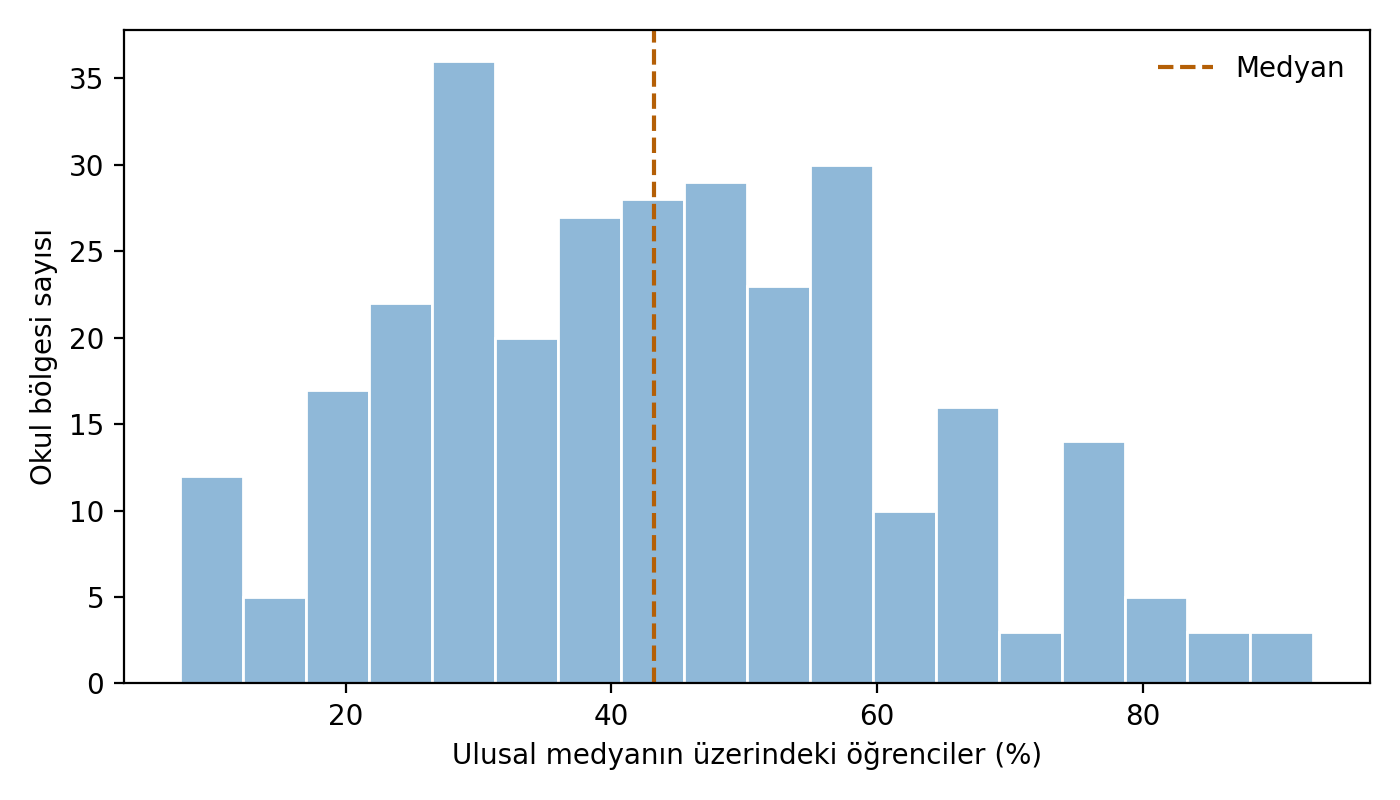
\includegraphics[width=\linewidth]{companion/outputs/figures/chapter03_star98_distribution.png}
\caption{B03 için paylaşılan Python histogramları ve kutu grafikleri.
Üst sıra yıl sonu notunu, alt sıra devamsızlık sayısını gösterir.}
\label{fig:b03-dogrulanmis-grafikler}
\end{figure}

\Needspace{22\baselineskip}
\begin{outputguidebox}
Tablo~\ref{tab:b03-dogrulanmis-betimsel} içinde not ortalaması 10,42,
medyanı 11'dir. Şekil~\ref{fig:b03-dogrulanmis-grafikler} içinde not
kutusunun sınırları 8 ve 14, bıyık uçları 0 ve 20'dir. Devamsızlık
dağılımında sağ kuyruk belirgindir; ortalama 5,71 iken medyan 4'tür.
Devamsızlık kutusu 0--8 aralığındadır; üst bıyık 20'ye uzanır,
daha yüksek değerler ayrı işaretlenir. Bu işaretler kayıtların hatalı
olduğunu tek başına göstermez.

Paylaşılan SPSS, R ve Python histogramlarının sınıf aralıkları farklı
olduğundan sütun yükseklikleri birebir eşleşmez. Karşılaştırılan kutu
grafiklerinde medyanlar, kutu sınırları ve bıyık uçları uyumludur;
işaret biçimleri ve gözlem etiketlerinin gösterimi farklıdır.
Hesapların uyumu örneklemin temsil gücünü kanıtlamaz.
Tablo~\ref{tab:b03-dogrulanmis-aralik} içindeki aralıkların daha geniş
bir evrene yönelik yorumu, örnekleme düzeni ve bağımsızlık gibi
çıkarım koşullarına bağlıdır; burada hesaplama uyumu doğrulanmıştır.
\end{outputguidebox}

\textbf{Raporlama örneği (doğrulanmış çıktılarla).}
``395 öğrencinin yıl sonu notu ortalaması 10,42, medyanı 11 ve standart
sapması 4,581 puandır. Devamsızlık sayısının ortalaması 5,71, medyanı 4
ve standart sapması 8,003'tür. Ortalama için hesaplanan yüzde 95
$t$ aralıkları sırasıyla 9,96--10,87 ve 4,92--6,50'dir. Sıfır notlu
38 kayıt korunmuş; devamsızlıkta 75'e ulaşan yüksek değerler grafiksel
incelemeye alınmış, otomatik olarak silinmemiştir. Sonuçlar daha geniş
bir öğrenci evrenine doğrudan genellenmemiştir.''


\textbf{Görev.} Not ve devamsızlık için birer grafik seçin. Aynı ölçeğe
sahip olmayan değişkenleri yalnız standart sapmalarını karşılaştırarak
``daha değişken'' ilan etmenin sakıncasını tartışın.

\section{R ile çözümlü uygulama}
\label{sec:r-b03}

\textbf{Soru.} Çalışma süreleri 2, 3, 3, 4 ve 13 saat olan örnekte merkez,
yayılım ve aykırı değer sınırlarını bulun. Bölümde kullanılan doğrusal
enterpolasyonla uyum için yüzdelik hesabında \texttt{type = 7} seçin.

\begin{lstlisting}[style=prismR]
saat <- c(2, 3, 3, 4, 13)
ceyrek <- quantile(saat, c(0.25, 0.75), type = 7)
ceyrek_acikligi <- IQR(saat, type = 7)
c(ortalama = mean(saat), medyan = median(saat),
  varyans = var(saat), standart_sapma = sd(saat))
quantile(saat, c(0, 0.25, 0.5, 0.75, 1), type = 7)
sinir <- c(ceyrek[1] - 1.5 * ceyrek_acikligi,
           ceyrek[2] + 1.5 * ceyrek_acikligi)
sinir
saat[saat < sinir[1] | saat > sinir[2]]
hist(saat, breaks = c(0, 3, 6, 9, 12, 15), right = FALSE,
     main = "Calisma suresi", xlab = "Saat")
boxplot(saat, horizontal = TRUE, xlab = "Saat")
c(ortalama_13_haric = mean(saat[saat != 13]),
  medyan_13_haric = median(saat[saat != 13]))
\end{lstlisting}

\begin{outputguidebox}
\textbf{Çözüm ve kontrol değerleri.} Ortalama 5, medyan 3, örneklem
varyansı 20,5 ve örneklem standart sapması 4,5277'dir. Beş sayı özeti
$(2;3;3;4;13)$; çeyrekler açıklığı 1; alt ve üst sınırlar 1,5 ve 5,5'tir.
13 saat üst sınırı aşar. Bu değer çıkarıldığında ortalama 3'e iner;
medyan 3 olarak kalır.
\end{outputguidebox}

\textbf{Yorum.} \texttt{sd} ve \texttt{var} örneklem hesabında $n-1$
bölenini kullanır. \texttt{boxplot} kutu sınırları için Tukey menteşelerini
kullanır; bunlar bu örnekte seçilen çeyreklerle aynıdır, her örneklemde aynı
olmak zorunda değildir. Aykırı değer işareti otomatik silme gerekçesi değildir.

\textbf{Pekiştirme ve yanıt.} 13'ü çıkarma işlemi yalnız duyarlılık
karşılaştırmasıdır. Ortalama iki saat değişirken medyanın değişmemesi,
medyanın bu uç değere karşı daha sağlam olduğunu gösterir.

\section{Bölüm özeti}

\begin{itemize}
  \item Grafik türü değişkenin ölçme düzeyine ve araştırma sorusuna göre seçilir.
  \item Ortalama tüm değerlere, medyan sıralamaya dayanır ve aykırı değerlere daha dayanıklıdır.
  \item Standart sapma ortalama çevresindeki, IQR orta yüzde 50'deki yayılımı özetler.
  \item Betimsel analiz eksik veri, çarpıklık ve aykırı değer incelemesini de içerir.
  \item Aynı merkeze sahip dağılımlar çok farklı yayılım ve biçim gösterebilir.
  \item Grafik eksenleri, sınıf aralıkları ve etiketler görsel yorumu
  çarpıtmayacak biçimde düzenlenmelidir.
\end{itemize}

\section*{Alıştırmalar}

\begin{enumerate}
  \item Ortalama ile medyanın belirgin biçimde ayrıldığı bir veri seti kurun.
  \item Hangi durumda standart sapma, hangi durumda IQR raporlayacağınızı açıklayın.
  \item Bir aykırı değeri silmeden önce sorulması gereken üç soruyu yazın.
  \item $3,4,4,5,9$ verisi için ortalama, medyan ve açıklığı hesaplayın.
  \item $10,12,12,13,15,28$ verisinin beş sayı özetini ve IQR değerini bulun;
  aykırı değer sınırlarını hesaplayın.
  \item Aynı ortalamaya fakat farklı standart sapmaya sahip iki küçük veri
  seti oluşturun ve dağılımlarını yorumlayın.
  \item 50 öğrencinin 20'si yüz yüze, 18'i karma ve 12'si çevrim içi eğitimi
  tercih ediyorsa frekans-yüzde tablosunu oluşturun.
  \item Histogram ile çubuk grafiği arasındaki üç temel farkı açıklayın.
  \item Sağa çarpık bir gelir dağılımında ortalama ile medyanın beklenen
  ilişkisini ve hangi özetin daha uygun olduğunu belirtin.
  \item Bir yazılım çıktısında toplam örneklem 200, geçerli gözlem sayısı 184
  ise analizden önce hangi kontrollerin yapılması gerektiğini yazın.
  \item Dikey ekseni 90'dan başlayan bir başarı yüzdesi grafiğinin oluşturacağı
  algı sorununu açıklayın ve uygun grafik düzenini önerin.
  \item Aykırı değer içeren bir veri seti için gözlem dâhil ve hariç betimsel
  özetleri karşılaştıran kısa bir duyarlılık analizi planlayın.
\end{enumerate}